\section{LTI系统的频域分析}

\subsection[虚指数函数作用于LTI系统的响应]{虚指数函数$e^{j\omega t}$作用于LTI系统的响应}

\begin{BoxDefinition}[频率响应函数]
    设LTI系统的冲激响应为$h(t)$,当激励为$e^{\mathrm{j}\omega t}$\footnote{幅度为1的虚指数函数}时,其零状态响应为
    \begin{Equation}
        y(t) = h(t)*e^{\mathrm{j}\omega t} = \int_{-\infty}^{\infty} h(\tau)e^{\mathrm{j}\omega(t-\tau)}d\tau = \int_{-\infty}^{\infty} h(\tau) e^{-\mathrm{j}\omega \tau} d\tau \cdot e^{\mathrm{j}\omega t}
    \end{Equation}
    其中$\int_{-\infty}^{\infty} h(\tau) e^{-\mathrm{j}\omega \tau} d\tau$正好为$\mathscr{F}\left[h(t)\right]$,记为$H(\mathrm{j}\omega)$,称为系统的频率响应函数,即
    \begin{Equation}
        y(t) = H(\mathrm{j}\omega) e^{\mathrm{j}\omega t}
    \end{Equation}
    $H(\mathrm{j}\omega)$反应了$y(t)$的幅度和相位随频率的变化。
\end{BoxDefinition}

\subsection{一般信号\texorpdfstring{$f(t)$}作用于LTI系统的响应}

\begin{BoxProperty}[傅里叶变换频域分析法]
    由LTI系统的齐次性和可加性可知,一般信号$f(t)$作用于系统的时候,响应满足
    \begin{Equation}
        \frac{1}{2\pi} \int_{-\infty}^{\infty} F(\mathrm{j}\omega) e^{\mathrm{j}\omega t}d\omega \longleftrightarrow \frac{1}{2\pi} \int_{-\infty}^{\infty} H(\mathrm{j}\omega)F(\mathrm{j}\omega) e^{\mathrm{j}\omega t} d\omega
    \end{Equation}
    即
    \begin{Equation}
        f(t) \longleftrightarrow y(t) = \mathscr{F}^{-1} \left[F(\mathrm{j}\omega)H(\mathrm{j}\omega)\right]
    \end{Equation}
    \begin{Equation}
        Y(\mathrm{j}\omega) = F(\mathrm{j}\omega) H(\mathrm{j}\omega)
    \end{Equation}
    因此频率响应可以定义为
    \begin{Equation}
        H(\mathrm{j}\omega) = \frac{Y(\mathrm{j}\omega)}{F(\mathrm{j}\omega)}
    \end{Equation}
    \begin{Equation}
        H(\mathrm{j}\omega) = \left|H(\mathrm{j}\omega)\right|e^{\mathrm{j}\theta(\omega)} = \frac{|Y(\mathrm{j}\omega)|}{|F(\mathrm{j}\omega)|}e^{\mathrm{j}\left[\varphi_y(\omega) - \varphi_f(\omega)\right]}
    \end{Equation}
    $|H(\mathrm{j}\omega)|$称为幅频响应(幅频特性),$\theta(\omega)$称为相频响应(相频特性)。

    $|H(\mathrm{j}\omega)|$是$\omega$的偶函数,$\theta(\omega)$是$\omega$的奇函数。
\end{BoxProperty}

\begin{BoxProperty}[指数形式傅里叶级数频域分析法]
    设LTI系统的激励为$f_T(t) = \sum\limits_{n=-\infty}^{\infty} F_ne^{\mathrm{j}n\Omega t}$,则响应
    \begin{Equation}
        y(t) = h(t) * f_T(t) =  \sum\limits_{n=-\infty}^{\infty} F_n\left[h(t) * e^{\mathrm{j}n\Omega t}\right] = \sum\limits_{n=-\infty}^{\infty} F_n H(\mathrm{j}\omega)e^{\mathrm{j}n\Omega t}
    \end{Equation}
    因此
    \begin{Equation}
        Y_n = F_n H(\mathrm{j}n\Omega)
    \end{Equation}
    即
    \begin{Equation}
        y(t) = \sum\limits_{n=-\infty}^{\infty} F_nH(\mathrm{j}n\Omega) e^{\mathrm{j}n\Omega t}
    \end{Equation}
\end{BoxProperty}


\begin{BoxProperty}[三角函数形式傅里叶级数频域分析法]
    设LTI系统的激励为$f_T(t) = \frac{A_0}{2} + \sum\limits_{n=1}^{\infty} A_n\cos(n\Omega t + \varphi_n)$,频率响应函数为$H(\mathrm{j}\omega) = |H(\mathrm{j}\omega)|e^{\mathrm{j}\theta(\omega)}$则响应
    \begin{Equation}
        y(t) = \frac{A_0}{2}H(0) + \sum\limits_{n=1}^{\infty} A_n|H(\mathrm{j}n\Omega)| \cos\left[n\Omega t + \varphi_n + \theta(\omega)\right]
    \end{Equation}
\end{BoxProperty}

\subsection[频率响应的求法]{频率响应$H(j\omega)$的求法}

\begin{BoxProperty}[已知微分方程求解频率响应]
    方程两边同时取傅里叶变换,可得$H(\mathrm{j}\omega)$关于$Y(\mathrm{j}\omega)$和$F(\mathrm{j}\omega)$的方程。

    移项即可得$H(\mathrm{j}\omega) = \frac{Y(\mathrm{j}\omega)}{F(\mathrm{j}\omega)}$

    根据$Y(\mathrm{j}\omega) = H(\mathrm{j}\omega)F(\mathrm{j}\omega)$可以进一步求响应$y(t)$。
\end{BoxProperty}

\begin{BoxProperty}[已知电路求解频率响应]
    根据电路列出$H(\mathrm{j}\omega) = \frac{Y(\mathrm{j}\omega)}{F(\mathrm{j}\omega)}$,标出电路各元件的阻抗即可根据各回路列方程解得所需比值。

    电感元件阻抗$\mathrm{j}\omega L$,电容元件阻抗$\frac{1}{\mathrm{j}\omega C}$,电阻元件阻抗$R$。
\end{BoxProperty}

\subsection{无失真传输与滤波}

\begin{BoxDefinition}[无失真传输]
    无失真传输是指输出信号和输入信号相比,信号只有幅度的大小和出现的时间先后不同,没有波形上的变化。设输入信号为$f(t)$,即满足
    \begin{Equation}
        y(t) = Kf(t-t_d)
    \end{Equation}
    频谱关系满足
    \begin{Equation}
        Y(\mathrm{j}\omega) = K e^{-\mathrm{j}\omega t_d}F(\mathrm{j}\omega)
    \end{Equation}
    无失真传输满足以下条件
    \begin{Equation}
        h(t) = K\delta(t-t_d)
    \end{Equation}
    \begin{Equation}
        H(\mathrm{j}\omega) = \frac{Y(\mathrm{j}\omega)}{F(\mathrm{j}\omega)} = Ke^{-\mathrm{j}\omega t_d}
    \end{Equation}
    即
    \begin{Equation}
        |H(\mathrm{j}\omega)| = K,\quad \theta(\omega) = -\omega t_d
    \end{Equation}

    \begin{Figure}[无失真传输幅频相频特性]
        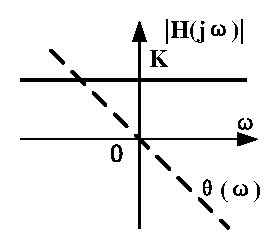
\includegraphics[width=30mm]{visio/4.11.pdf}
    \end{Figure}

    根据输入信号判断输出信号是否失真只需要看输入信号的各次谐波频率对应的$|H(\mathrm{j}\omega)|$是否相等,$\theta(\omega)$的值是否在同一条过原点的直线上(即保证$t_d$相同)即可。

    系统的群时延为
    \begin{Equation}
        \tau = -\frac{d\theta(\omega)}{d\omega}
    \end{Equation}

\end{BoxDefinition}

\begin{BoxDefinition}[失真相关概念]
    幅度失真是指各频率分量幅度产生不同程度衰减。

    相位失真是指各频率分量产生的相移不与频率成正比,使各频率分量在时间轴上的相对位置发生变化。

    线性失真是指只存在幅度或相位失真,不产生新的频率成分。

    非线性失真是指产生新的频率成分的失真。
\end{BoxDefinition}

\begin{BoxDefinition}[理想低通滤波器]
    具有如下图所示的幅频相频特性的系统称为理想低通滤波器。
    \begin{Figure}[理想低通滤波器幅频相频特性]
        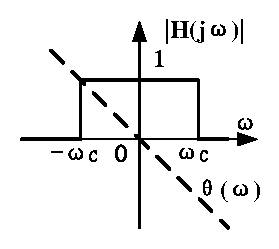
\includegraphics[width=30mm]{visio/4.12.pdf}
    \end{Figure}

    $\omega_c$称为截止角频率,频率响应可以写为

    \begin{Equation}
        H(\mathrm{j}\omega) =
        \left\{
        \begin{aligned}
            e^{-\mathrm{j}\omega t_d} & , & |\omega| < \omega_c \\
            0                         & , & |\omega| > \omega_c
        \end{aligned}
        \right. = g_{2\omega_c}(\omega)e^{-\mathrm{j}\omega t_d}
    \end{Equation}
    理想低通滤波器的冲激响应为
    \begin{Equation}
        h(t) = \mathscr{F}^{-1}\left[H(\mathrm{j}\omega)\right] = \mathscr{F}^{-1}\left[g_{2\omega_c}(\omega)e^{-\mathrm{j}\omega t_d}\right] = \frac{\omega_c}{\pi} \mathrm{Sa}\left[\omega_c(t-t_d)\right]
    \end{Equation}
    显然不是因果系统,因此理想低通滤波器不存在。

    理想低通滤波器的阶跃响应
    \begin{Equation}
        g(t) = h(t) * \varepsilon(t) = \int_{-\infty}^{t} \frac{\omega_c}{\pi} \frac{\sin\left[\omega_c(\tau-t_d)\right]}{\omega_c(\tau-t_d)}d\tau = \frac{1}{2} + \frac{1}{\pi}\int_{0}^{\omega(t-t_d)}\frac{\sin x}{x} dx
    \end{Equation}
    定义正弦积分为
    \begin{Equation}
        Si(x) = \int_{0}^{y} \frac{\sin x}{x} dx
    \end{Equation}
    则阶跃响应可以写为
    \begin{Equation}
        g(t) = \frac{1}{2} + \frac{1}{\pi}Si\left[\omega_c(t-t_d)\right]
    \end{Equation}
    \begin{Figure}[理想低通滤波器的阶跃响应]
        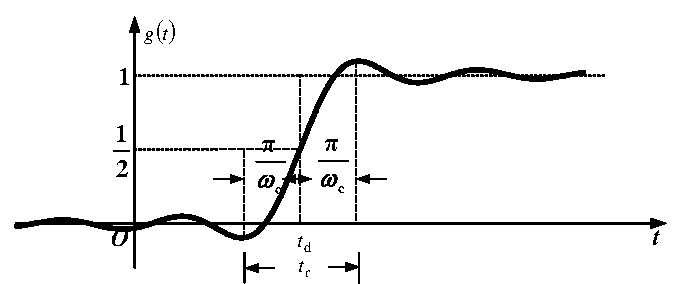
\includegraphics[width=60mm]{visio/4.13.pdf}
    \end{Figure}
    其中最小值位置为$t_d-\omega$,最大值位置为$t_d+\omega$,上升时间$t_r = 2\cdot\frac{\pi}{\omega_c}$。

    $g_{max}(t) = \frac{1}{2} + \frac{\mathrm{Si}(\pi)}{\pi} = 1.0895$

    显然,只要$\omega_c<\infty$,必有振荡,该由频率截断效应引起的振荡称为吉布斯现象。
\end{BoxDefinition}

\begin{BoxProperty}[物理可实现系统条件]
    从时域特性上来说,物理可实现系统的冲激响应满足
    \begin{Equation}
        h(t)=0,\quad t<0
    \end{Equation}
    从频域特性来说,满足佩利-维纳准则(必要条件)
    \begin{Equation}
        \int_{-\infty}^{\infty} |H(\mathrm{j}\omega)|^2d\omega<\infty
    \end{Equation}
    且
    \begin{Equation}
        \int_{-\infty}^{\infty}\frac{\left|\ln|H(\mathrm{j}\omega)|\right|}{1+\omega^2}d\omega<\infty
    \end{Equation}
    从该准则可看出,对于物理可实现系统,其幅频特性可在某些孤立频率点上为$0$,但不能在某个有限频带内为$0$。
\end{BoxProperty}